\begin{figure}[ht]
    \centering
    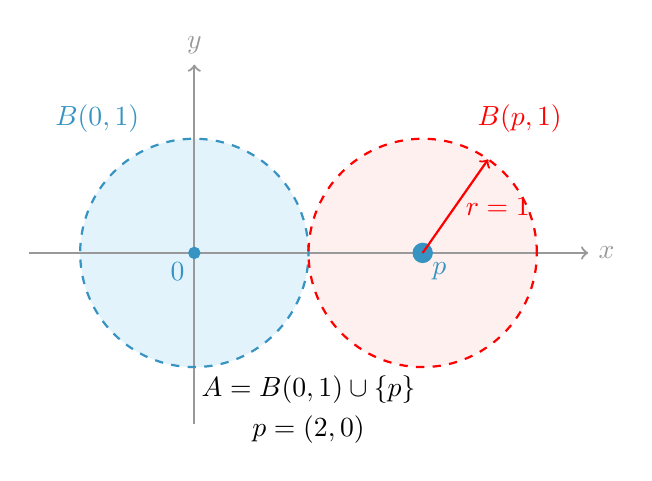
\begin{tikzpicture}[scale=1.45]
        % O conjunto A e formado pela bola B(0,1) e pelo ponto p.
        \path[fill=Cerulean!12] (0,0) circle (1);
        \path[fill=Red!6] (2,0) circle (1);

        \draw[->, gray!80, thick] (-1.45,0) -- (3.45,0) node[right] {$x$};
        \draw[->, gray!80, thick] (0,-1.5) -- (0,1.65) node[above] {$y$};

        \draw[Cerulean!80!black, thick, dashed] (0,0) circle (1);
        \draw[Red, thick, dashed] (2,0) circle (1);

        \filldraw[Cerulean!80!black] (0,0) circle (1.4pt) node[below left] {$0$};
        \filldraw[Cerulean!80!black] (2,0) circle (2.4pt) node[below right] {$p$};

        \draw[Red, thick, ->] (2,0) -- ++(55:1)
            node[midway, right] {$r=1$};

        \node[Cerulean!80!black] at (-0.85,1.18) {$B(0,1)$};
        \node[Red] at (2.85,1.18) {$B(p,1)$};
        \node at (1,-1.2) {$A=B(0,1)\cup\{p\}$};
        \node at (1,-1.55) {$p=(2,0)$};
    \end{tikzpicture}
    \caption{O ponto $p=(2,0)$ é isolado em $A=B(0,1)\cup\{(2,0)\}$.}
\end{figure}
